\chapter*{The neuroanatomical signature of time in Working Memory}

% Il m'a fallu un temps conséquent pour me former au début du stage à l'analyse en EEG. 
% Au MVA, j'avais déjà fait des neurosciences, ainsi que la théorie physique des EEG et MEG à l'aide du cours d' \href{http://math.ens-paris-saclay.fr/version-francaise/formations/master-mva/contenus-/imagerie-fonctionnelle-cerebrale-et-interface-cerveau-machine-161979.kjsp?RH=1242430202531}{Imagerie fonctionnelle cérébrale et interface cerveau machine}, au cours duquel j'ai déjà manipulé les interfaces cerveau machines par exemple en
% \href{https://github.com/crsegerie/bci_competition}{réimplémentant} la solution des vainqueurs de la compétition \href{https://www.kaggle.com/c/inria-bci-challenge}{inria-bci-challenge}. Mais en réalité, lors de cette compétition kaggle, les participants ont été épargnés du préprocessing du traitement de la donnée des EEG : les organisateurs du kaggle avaient déjà nettoyé la donnée qui était alors utilisable par n'importe quel praticien en machine learning. Mais il existe tout un savoir faire afin de nettoyer la donnée, et ce nettoyage et cette analyse est presque plus technique que du machine learning conventionnel.



% \begin{comment}
% \section{Théorie}
% voir le cours de gramfort. Voir le cours du mva.
% \section{L'écosysteme MNE - Bids}
% \subsection{mne-python}
% \subsection{mne-bids-pipeline}
% \subsection{mne-bids}
% \end{comment}


\section*{Prelude}

I divided this report into two parts that roughly follow the chronological order of my internship.

The first chapter gives the scientific context of my internship. This part is an account of the environment in which I am inserted and of the knowledge required to understand my work hereafter. Scientific activity is no longer a solitary activity, especially in neuroscience, where the tools used are based on years of collective work. I notably explain in this chapter the ins and outs of the pilot study paper \cite{herbst2021abstracting} on which I rely. The goal of my internship is to complete this pilot study by analyzing magnetoencephalography (MEG) data, by finding appropriate mathematical methods to analyze the MEG data, and to implement these mathematical methods in an open source automatic analysis pipeline, the mne-bids-pipeline. This pipeline aims to allow future cognitive science researchers to analyze electroencephalogram data in a snap, while promoting replicability and open science. This part could constitute the introduction part of a future paper.

The second chapter is an exhibition of my work. We reproduced the results of the pilot study but using MEG imaging to analyze the parts of the brain at work during the use of working memory. We used the mne-bids-pipeline to analyze the data. But we had to adapt the mne-bids-pipeline by using new algorithms in order to meet the requirements of our experimental paradigm. An important part of my work has been allocated to implement in open-source these methods rigorously, while optimizing the computation time. This part could constitute the method, results and discussion part of a future paper.

\chapter{Scientific Context}

Potentiellemnt dire : developper des methodes mathematiques qui vont permettre à la suite aux chercheurs d'utiliser la pipeline pour open sscience... Dire que nous avons pu égalemetn eu des premiers résultats afin de trouver les régions du cervaux, même si ce n'était pas le but premier de mon stge, une early analyse sous le prismes des sciences cognitive à été menée.

This internship combines two aims: to extract the neural signatures of time stored in working memory from existing MEG data, and to contribute to ongoing efforts of establishing an open-science pipeline for MEG analysis in BIDS (standardized brain imaging data format, \cite{gorgolewski2016brain}). The project is part of a collaboration between NeuroSpin, and the MNE Python developers at Inria, with the aim to push the use of BIDS for more transparent and open MEEG research practices.

As shown by a large number of studies, humans can perceive temporal intervals (durations in the range of seconds), judge or compare them with other intervals, and recognize or reproduce them later on. Hence, durations can be stored in memory, like sensory stimuli. It is however not known yet how the brain achieves this, for instance in which format (continuous or symbolic) durations are stored and which brain mechanisms support this ability \cite{polti2018effect}, \cite{teki2014working}. In this internship, I joined the inria/neurospin team in the ongoing analysis of the previously collected MEG data, with the aim to reconstruct source time courses of brain activity from the cortex, and possibly the hippocampus and cerebellum \cite{gauthier2020hippocampal} using volume source models in MNE-Python.

The pipeline developed during the project will contribute to ongoing open-science
efforts by the team to establish a robust and publicly available pipeline for source
reconstruction of MEEG data based on the BIDS MEG data format in MNE-Python.


% Mes connaissances préalables: MVA cours imagerie fonctionnelel cerebrale + Neuroscience + imagerie médiacle


\section{The Time in Working Memory (TiWM) paradigm}

Cette partie présente the \textit{time in Working Memory} paradigm, qui a été exposé dans le papier \cite{herbst2021abstracting}. Le but de mon stage est d'aider à la reproduction de ce papier mais cette fois ci en utilisant des donnée venant de MEG.

\subsection{Paradigme de la Pilot study: Abstracting Time in Working Memory}

Planning for the future relies on the ability to remember the duration of events, but it is unknown how durations are stored in the brain's working memory.  The paper abstracting time in working memory proposes a new n-item delayed duration reproduction task to assess whether elapsed time is stored in memory as a continuous feature or as an abstract element. [present the clock models, but say that it is outside the spope of my internship. My training as a mathematician does not give me the tools to interpret the results, but simply through dialogue with the cognitive researchers, I propose mathematical methods].The participants listened to sequences composed of empty time intervals that they had to reproduce as precisely as possible. For each sequence, one can manipulate the number of time intervals and the overall duration of the sequence to separate their effects on recall accuracy.  Temporal reproduction accuracy decreased systematically with an increasing number of items. These results suggested that the number of time intervals, not their duration, determines recall precision. According to the brain clock models proposed by cognitive science, these results are interpreted as evidence of the existence of a symbolic representation of duration in working memory.

Thus, according to this preliminary study, we know that durations are not represented in a continuous way, but in a symbolic way. But we still do not know in which part of the brain the information is stored. In order to visualize in which part of the brain the working memory is encoded, we reproduced the experiment this time by recording the cerebral data with magnetoencephalograms. In this new experiment, we no longer concentrate on the analysis of the accuracy of the restitution of the duration of the time intervals, but we will concentrate more on the visualization of the frequencies and cerebral areas at stake for the working memory.


\subsection{Dataset description}


Nombre de participants


\begin{figure}[ht]
    \centering
    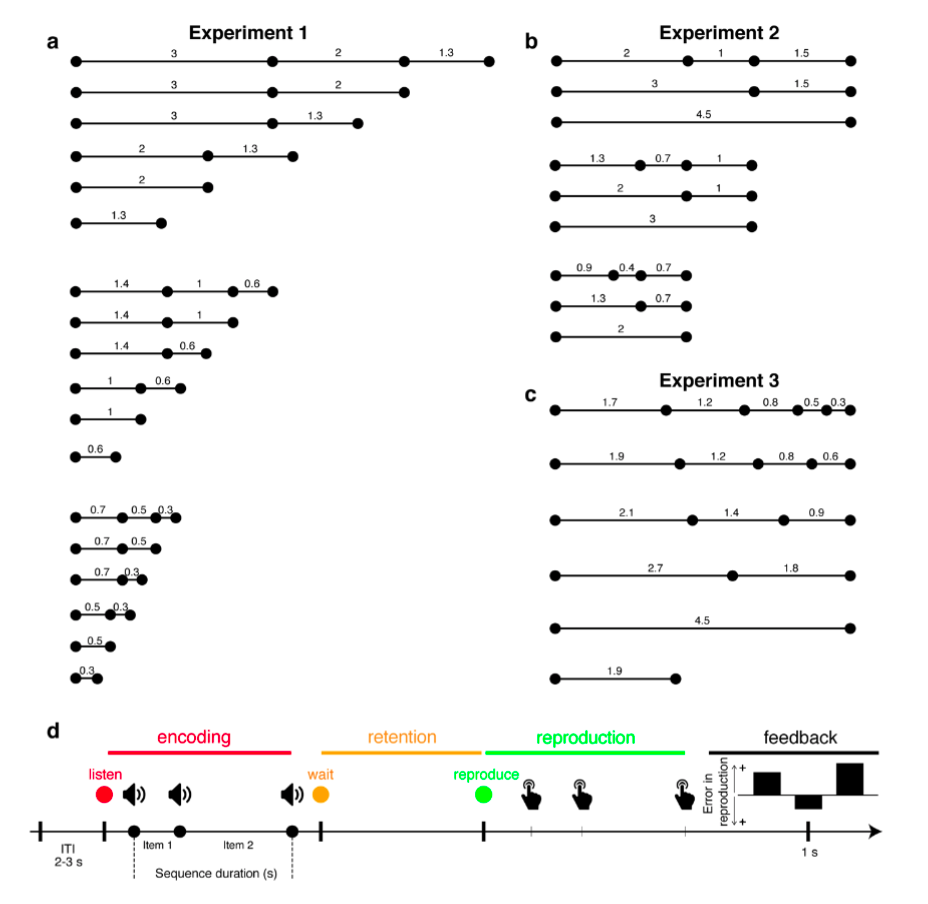
\includegraphics[width=10cm]{images_report/n-item delayed reproduction task.png}
    \caption[n-item delayed reproduction task]%
    {n-item delayed reproduction task - Panels a–c depict the individual items and sequences used in Experiment 1, 2, and 3, respectively. Black dots represent 1kHz tones. All numbers are durations in seconds. (a) The set of sequences used in Experiment 1, in which the number of items in a sequence and the full sequence duration covaried. A sequence was composed of 1, 2 or 3 items, and its duration varied from 0.3s to 6.3 s. (b) In Experiment 2, the number of items and the sequence duration were orthogonalized. A sequence was composed of 1, 2 or 3 items with sequence duration fixed to 2 s, 3 s, or 4.5 s irrespective of the number of items composing it. (c) In Experiment 3, a sequence was composed of 1 to 5 items. Only two sequence durations were used (1.9 s and 4.5 s). (d) Example trial. In all experiments, each trial was composed of four phases: First, participants listened to a sequence of pure tones demarcating time intervals of varying duration. Following a retention interval, participants were asked to reproduce the temporal sequence as precisely as possible. In the example depicted here, the sequence was composed of two items. Following the reproduction (green), feedback was provided showing the relative temporal reproduction error for teach item in the sequence.}

    \label{paradigm}
\end{figure}

In Experiment 2 (Fig. 1B), the number of items and the duration of the sequence were orthogonalized. Three sequence durations were tested (2 s, 3 s and 4.5 s) and the number of items was 1, 2 or 3 items for each sequence. Wit

- Les modèles de clocks cerebrales??
- Pourquoi EEG plutot que FMRI

\subsection{Donner le but du Stage}

Reproduire cette study mais avec la MEG. Nous ne smme interessé que par l'experiment 2 puisqu'il faut que l'on garde constant la durée du signal.
D'autre part, afin de maximiser la significativité du signal , nous n'utilions uniquement des event  comportant 1 ou 3 items, cela afin de maximiser la puissance de la statistique étant donné que la pilot study à montré que la relation est linéaire.

\subsection{Glossaire}

\begin{table}[ht]
    \centering
    \begin{tabular}{@{}| p{4cm}|p{9cm}| @{}}
        \hline
        EEG-MEG                     & The Electro-magnetoencephalography is a non-invasive methods for studying brain function that reflect the electrical activity of neuronal populations with millisecond temporal resolution.                                                                                                                                                             \\

        Local field potential (LFP) & electric potential in the extracellular space around neurons. LFP is a widely available signal in many recording configurations, ranging from single-electrode recordings to multi-electrode arrays                                                                                                                                                     \\
        Neuronal oscillations       & prominent feature of spontaneous and task-related brain activity that occur at the level of single units, local field potentials (LFPs), and EEG/MEG recordings. The traditional view is that neuronal oscillations reflect inhibition-based fluctuations of neuronal activity that emerge from the synchronous activation of large neuronal ensembles. \\
        Spectral power              & reflects the amplitude of neural oscillations computed through a time–frequency transformation (TFT).                                                                                                                                                                                                                                                   \\
        \hline
    \end{tabular}
    \caption{Glossary of the Neural Oscillation and of the Theory of the working memory. \cite{roux2014working}}
    \label{Tab:Glossary_theory}
\end{table}

\begin{table}[ht]

    \centering
    \begin{tabular}{@{}| p{3cm}|p{10cm}| @{}}
        \hline
        Session      & A logical grouping of neuroimaging and behavioural data collected consistently across participants. A session includes the time involved in completing all experimental tasks. This begins when a participant enters the research environment until he/she leaves it.                                                    \\
        Run          & An uninterrupted period of continuous data acquisition without operator involvement.                                                                                                                                                                                                                                     \\
        Event        & An isolated occurrence of a presented stimulus, or a subject response recorded during a task                                                                                                                                                                                                                             \\
        Epoch        & In the MEEG literature, the term epoch designates the outcome of a data segmentation process. Typically, epochs in event-related designs (for analysis of event related potentials or event related spectral perturbations) are time-locked to a particular event (such as a stimulus or a response)                     \\
        Evoked data  & Evoked objects typically store an EEG or MEG signal that has been averaged over multiple epochs, which is a common technique for estimating stimulus-evoked activity.                                                                                                                                                    \\
        Sensors      & Sensors are the physical objects or transducers that are used to perform the analogue recording, i.e., EEG electrodes and MEG magnetometers/ gradiometers. Sensors are connected to amplifiers, which not only amplify, but also filter the MEEG activity.                                                               \\
        Channels     & Channels refer to the digital signals that have been recorded by the amplifiers. It is thus important to distinguish them from sensors. A ‘bad channel’ refers to a channel that is producing a consistently artifactual or low-quality signal.                                                                          \\
        Sensor space & Sensor space refers to a representation of the MEEG data at the level of the original sensors, where each of the signals maps onto the spatial location of one of the sensors.                                                                                                                                           \\
        Source space & Source space refers to MEEG data reconstructed at the level of potential neural sources that presumably gave rise to the measured signals (according to an assumed biophysical model). Each signal maps onto a spatial location that is readily interpretable in relation to individual or template-based brain anatomy. \\
        \hline
    \end{tabular}
    \caption{Glossary of MEEG terminology commonly used to describe stimulation and task parameters and protocols as defined in \cite{pernet2018best}}

    \label{Tab:Glossary_protocol}
\end{table}



\section{EEG, MEG}

EEG (electroencephalography) end MEG (magnetoencephalography) measures the electrical activity of our brain via electrodes that are placed on the scalp. It tells us, from the surface measurements, how active the brain is. It is possible to measure both eeg and meg data, so the acronym meeg is used to designate this data.

Pour notre paradigme experimental, il est bien plus important d'avoir une grande precesion temporelle, nous avons donc choisi d'utiliser les MEG de neurospin [image neurospin MEG], qui sont parmis les seuls MEG en France.


% http://meg-france.in2p3.fr/_lesCentres/Neurospin_en.php
The MEG lab is part of NeuroSpin, a neuroimaging center located on the campus of Saclay. We are part of the Comissariat à l'Energie Atomique (CEA), the Division of Life Sciences (DSV) and the Institute of BioImaging (I2BM) as well as the INSERM Cognitive Neuroimaging Unit.

Equipment
The MEG at Neurospin is an Elekta Neuromag 306 sensors whole-head device (details). The MEG helmet consists of 102 sensors-triplets (1 triplet = 2 orthogonal planar gradiometers and 1 magnetometer).


\subsection{How does EEG work?}

The brain is an electrical system – all of our thoughts (conscious or otherwise) are generated through a network of neurons, that send signals to each other with the help of electrical currents. The more electrical signals, the more neuronal communication, which corresponds to more brain activity.

The electrodes of an EEG headset can’t detect changes in single neurons, but instead detect the electrical changes of thousands of neurons signalling at the same time.

The signal from the electrodes is then sent to an amplifier, that (no surprises here) amplifies the signal. A computer then receives this signal, and can generate various maps of brain activity, with a rapid temporal resolution.

A drawback for EEG is the spatial resolution – as the electrodes measure electrical activity at the surface of the brain, it is difficult to know whether the signal was produced near the surface (in the cortex) or from a deeper region.

There are calculations that can be applied that attempt to get around this limitation (e.g. [2]), but it remains a challenge for EEG research.

\subsection{MEG in comparison to EEG}
Although EEG and MEG signals originate from the same neurophysiological processes, there are important differences.[28] Magnetic fields are less distorted than electric fields by the skull and scalp, which results in a better spatial resolution of the MEG. Whereas scalp EEG is sensitive to both tangential and radial components of a current source in a spherical volume conductor, MEG detects only its tangential components. Scalp EEG can, therefore, detect activity both in the sulci and at the top of the cortical gyri, whereas MEG is most sensitive to activity originating in sulci. EEG is, therefore, sensitive to activity in more brain areas, but activity that is visible in MEG can also be localized with more accuracy.

Scalp EEG is sensitive to extracellular volume currents produced by postsynaptic potentials. MEG detects intracellular currents associated primarily with these synaptic potentials because the field components generated by volume currents tend to cancel out in a spherical volume conductor.[29] The decay of magnetic fields as a function of distance is more pronounced than for electric fields. Therefore, MEG is more sensitive to superficial cortical activity, which makes it useful for the study of neocortical epilepsy. Finally, MEG is reference-free, while scalp EEG relies on a reference that, when active, makes interpretation of the data difficult.


\subsection{Generalities about MEG data and their preprocessing}

\begin{figure}[ht]
    \centering
    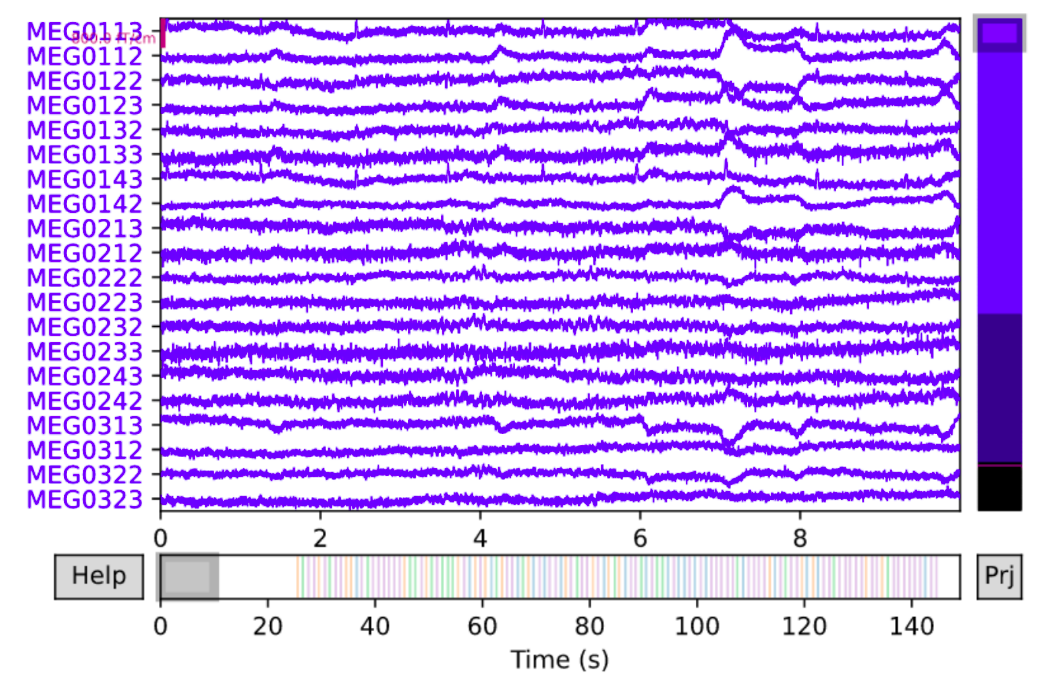
\includegraphics[width=10cm]{images_report/preprocessing/raw_data/Example_of_MEG_recording_reduced.png}
    \caption{Example of an MEG recording of a passive session. Here 20 of the 306 channels are represented.}
\end{figure}

With magnetoencaphalography we can capture the magnetic field created by the electrical currents in our brain. The MEG data are collected through two types of sensors : the gradiometers and the magnetometers. The MEG data I am manipulating during the internship are composed of 204 gradiometer channels and 102 magnetometer channels (Figure 1). These MEG data were recorded
trhough three sessions per subjects : one at rest with closed eyes, one passive with separately visual
and auditive stimuli and one with sensorimotor tasks (audio-visual stimuli with manual response)
([Taylor et al., 2017]).





\section{L'écosysteme MNE}

To realize analysis on MEG recordings I used the MNE-Python library \cite{GramfortEtAl2013a}.

Raw MEG data, epochs or evoked response can also be studied in the frequency domain. Nine
frequency bands are commonly used and are defined in Table \ref{Tab:neural_freq_band}.

\begin{table}[ht]
    \caption{Comparison of EEG bands for a typical adult}
    \centering
    \begin{tabular}{@{}| p{1.2cm}|p{2.5cm}| p{4.5cm}|p{4.5cm}| @{}}
        \hline
        Band  & Frequency (Hz) & Location                                       & Normally                                                                \\
        Delta & $\leq  4$      & frontally in adults, high-amplitude waves      & slow-wave sleep                                                         \\
        Theta & 4–8            & Found in locations not related to task at hand & Drowsiness or idling. Associated with inhibition of elicited responses. \\
        Alpha & 8–14           & posterior regions of head                      & relaxed, inhibition control                                             \\
        Beta  & 14–30          & mainly frontaly, low-amplitude waves           & active thinking, focus                                                  \\
        Gamma & $\geq 30$      & Somatosensory cortex                           & Cross-modal sensory processing or short-term memory                     \\
        \hline
    \end{tabular}
    \label{Tab:neural_freq_band}
\end{table}


mne python est une librairie python open-source permettant d'analyser les données cérébrales venant d'EEG ou de MEG. Le format BIds

\subsection{mne-python}


\begin{figure}[ht]
    \centering
    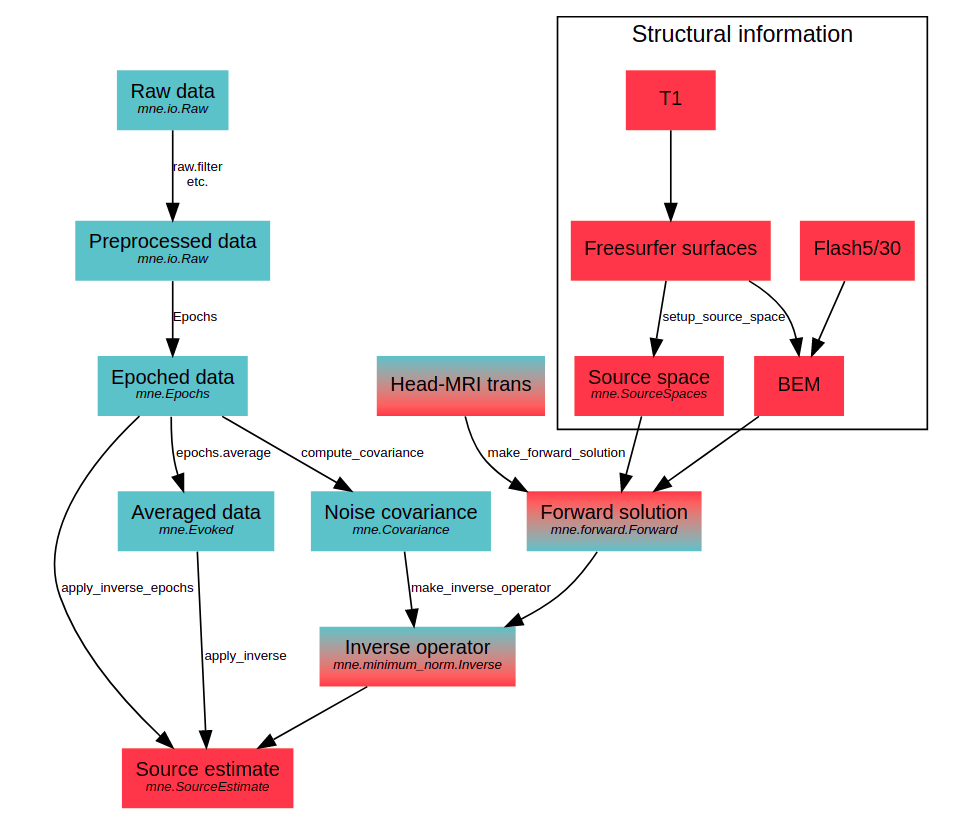
\includegraphics[width=10cm]{images_report/workflow_of_the_mne_software.png}
    \caption{Workflow of the MNE software \cite{GramfortEtAl2013a}}
\end{figure}


\subsection{the Brain Imaging Data Structure (BIDS) format}

The main objective of my internship was to extend the age prediction method I presented pre-
viously in order to apply it on new and diverse datasets. To begin with, I implemented the usage
of a standard electrophysiological data format called Brain Imaging Data Structure or BIDS. As
a second step, I made modifications in the script of the method to include the extraction of new
features and to ease the multimodal handling of the stacking regressor.

\begin{figure}[ht]
    \centering
    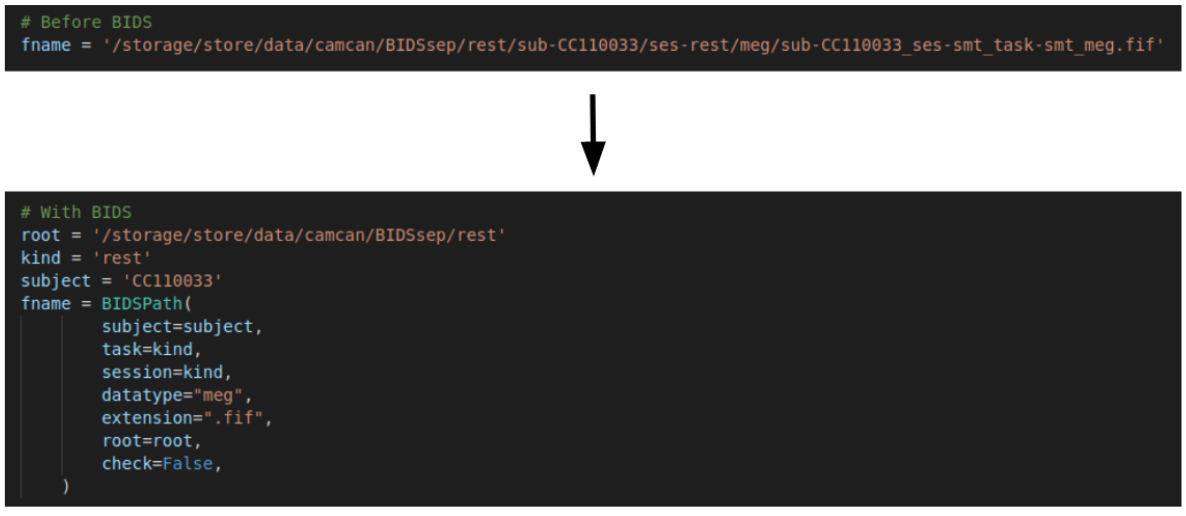
\includegraphics[width=10cm]{images_report/bids_example.png}
    \caption{Example of a modification made to use the script with BIDS-compatible datasets.}
    \label{bids_example}
\end{figure}

The Brain Imaging Data Structure was created to provide a simple way to organize neuroimaging data. The aim of this structure is to be a standard format to make the data accessible to every-one and avoid confusion. Thanks to a Python package called MNE-BIDS \cite{appelhoff2019mne}, datasets can easily be converted in the BIDS format. So, if datasets can be transformed in BIDS-compatible datasets, there is only need for the method to support datasets in this format.

Figure \ref{bids_example} illustrates one of the modifications I made to allow support of datatsets in BIDS format. Without any standard format, to access a file you need to write the whole path. One path is specific to one file so if you want to access another file or even another dataset you will need to change the whole path. If the dataset is in the BIDS format, it is possible to use the function BIDSPath of MNE-BIDS to call a file. In this case, if you want to call another file or another BIDS-compatible dataset you only need to change a few arguments of this function like the subject name or the file root and you do not have to think about the whole path. It also allows to use EEG data easily just by changing the parameter "datatype".

Thus, by implementing the support of BIDS format in the age-prediction model it is possible to switch between BIDS-compatible datasets by only modifying a few elements of the scripts even
if the datasets contain EEG instead of MEG data. We can now perform the analysis made in
\cite{herbst2021abstracting} on new datasets.


\subsection{Automatic preprocessing with the MNE-BIDS-Pipeline}

Using BIDS-compatible datasets enables us to apply the MNE-BIDS-Pipeline to the preprocessing part of the model. The MNE-BIDS-Pipeline is an automatic preprocessing and processing pipeline for MEG and EEG data stored following the BIDS format \cite{gorgolewski2016brain}. To apply the preprocessing steps wanted, the MNE-BIDS-Pipeline only requires to set the corresponding parameter in a configuration file. Once it is done for one dataset it can be used on other datasets just by changing one line in the configuration file.

The MNE-BIDS-Pipeline (\url{https://github.com/mne-tools/mne-bids-pipeline}) is still in development. As I wanted to use it for the time in working memory paradigm, I had to help implement the missing features I needed.

\begin{itemize}
    \item I Added the possibility to exclude runs from the analysis.
    \item Files docstrings in the preprocessing steps were updated.
    \item Warn if using ICA and no EOG- or ECG-related ICs were detected.
    \item Added the possibility to have different runs for different subjects.
    \item Massive PR
    \item The sanity check comparing the rank of the experimental data and the rank of the empty-room after Maxwell-filtering did not use the maxfiltered data.
    \item Some variables were named incorrectly in some test config files.
\end{itemize}

(\url{https://raw.githubusercontent.com/mne-tools/mne-bids-pipeline/main/docs/source/changes.md}).
In the case of time in working memory parafdigm, it is very useful to employ this pipeline because:
\begin{itemize}
    \item it will be exactly the same steps for all the datasets.
    \item It enhances reproducibility, because we now only nned a simple configuration file to reproduce every figure.
    \item The most classical steps of preprocessing and analysis of MEEG studies are common to all studies, and it is enough to change one or two scripts to obtain a complete study.
    \item De nombreux meta parammetres sont dur à calibrer, notemment pour le nettoyage et lors du passage dans l'espace des source, et sans expertise, il vaut mieux utiliser les parametres par défaults utilisés dans la pipeline
    \item La pipeline permet de process les différents participants en paralleles, ce qui permet de considérablement accellerer les temps de calculs.
\end{itemize}
